\documentclass[10pt,a4paper]{article}
\usepackage[utf8]{inputenc}
\usepackage{amsmath}
\usepackage{amsfonts}
\usepackage{amssymb}
\usepackage{graphicx}
\usepackage{float}
\usepackage{tabu}
\author{Akhilesh Kumar (201351009) \\ Gaurav Tolani 201352021}
\title{Parallel Programming (CS403)\\ Project-1\\Simulation of Brownian Movement of a Stock Price}
\begin{document}
\maketitle
\tableofcontents
\newpage
\section{Problem Statement}
\subsection{What is Brownian Movement?}
Standard definition of Brownian motion is:
\begin{quote}
Brownian motion is the random motion of particles suspended in a fluid (a liquid or a gas) resulting from their collision with the fast-moving atoms or molecules in the gas or liquid.\end{quote}
Dwelling into probability and statistics, Brownian motion is among the simplest of the continuous-time stochastic (or probabilistic) processes.\\
In mathematics, the Wiener process is a continuous-time stochastic process named in honor of Norbert Wiener. It is often called standard Brownian Motion.
\subsection{What is Monte Carlo Simulation?}
Monte Carlo methods (or Monte Carlo experiments) are a broad class of computational algorithms that rely on repeated random sampling to obtain numerical results. Their essential idea is using randomness to solve problems that might be deterministic in principle.\\
A Monte Carlo simulation is an attempt to predict the future many times over. At the end of the simulation, thousands or millions of "random trials" produce a distribution of outcomes that can be analyzed.\\
\subsection{Geometric Brownian Motion}
A geometric Brownian motion (GBM) (also known as exponential Brownian motion) is a continuous-time stochastic process in which the logarithm of the randomly varying quantity follows a Brownian motion (also called a Wiener process) with drift. It is an important example of stochastic processes satisfying a stochastic differential equation (SDE); in particular, it is used in mathematical finance to model stock prices in the Black–Scholes model.\\
The geometric Brownian motion (GBM) is the most basic processes in financial modelling.\\
The formula for GBM is found below, where ``S" is the stock price, ``$\mu$" (the Greek mu) is the expected return,``$\sigma$" (Greek sigma) is the standard deviation of returns, ``t" is time, and ``$\varepsilon$" (Greek epsilon) is the random variable:\\
\begin{equation}
\frac{\Delta S}{S}=\mu t + \sigma \varepsilon \sqrt{\Delta t}
\end{equation}
If we change and rearrange the formula and take log of the above equation on both sides, the final equation which we will get is:\\
\begin{equation}
S(t)=S(0)e^{(\mu - \sigma ^{2}/2)t + \sigma W(t)}
\end{equation}
where,
W(t)=$Brownian Motion, \sqrt{t} z(t) $, and \\
z(t)=normal random variable b/w 0 and 1 with mean=1 and variance=t\\
In this problem, we will try to simulate the Brownian motion of a stock price for a given time using Monte Carlo simulations for different number of iterations and parallelize the algorithm to see the performance change.
\section{Algorithm Used}
An algorithm for simulating the stock price at time t>0, given that current price at time t=0 is $S_{0}$ is as follows:\\
\begin{enumerate}
\item Generate random variable z ~N(0,1)
\item Set $\mu_{t}=(\mu - \sigma^{2}/2)t$ and $\sigma_{t}=\sigma t^{0.5}$
\item Set $S_{t}=S_{0} \times e^{\mu_{t} + \sigma_{t} z}$
\end{enumerate}
\section{Output}
\subsection{Language Used}
Due to time constraint, for the time being, we have implemented the serial code on the language R and C. R is a programming language and software environment for statistical computing and graphics supported by the R Foundation for Statistical Computing. The R language is widely used among statisticians and data miners for developing statistical software and data analysis.\\
Because of the some inbuilt features which R provide (eg. inbuilt function for generating random variable and graph plotting), the effort for making code was considerably reduced.
\subsection{Outputs(Graphs and execution time for 'R')}
Given the parameters,\\
$S_{0}$, initial price of stock= 10,\\
$\mu$, expected return=13\%,\\
$\sigma$, standard  deviation of returns=15\%,\\
time, t=100
\begin{enumerate}
\item For 100 simulations,\\
\begin{figure}[h]
\centering
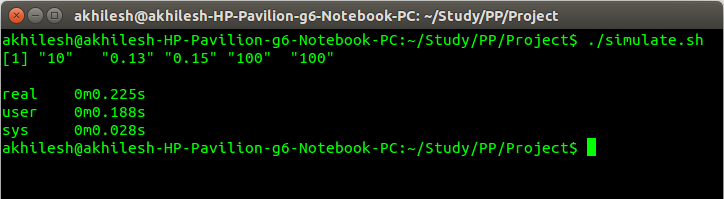
\includegraphics[scale=0.5]{100}
\caption{Execution time for 100 simulations}
\end{figure}
\begin{figure}[h]
\centering
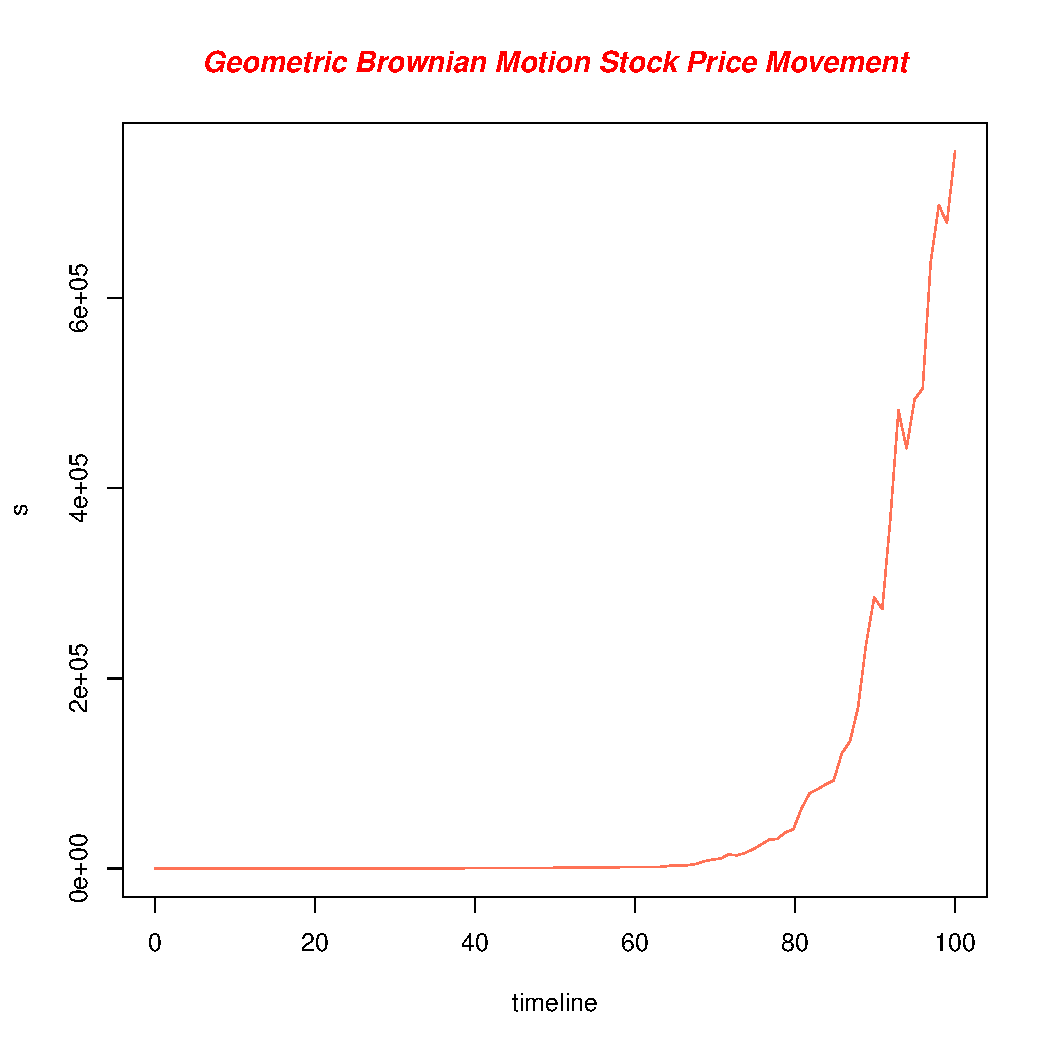
\includegraphics[scale=0.5]{100_graph.pdf}
\caption{Brownian motion graph for 100 simulations}
\end{figure}

\newpage
\item For 1000 simulations,\\
\begin{figure}[h]
\centering
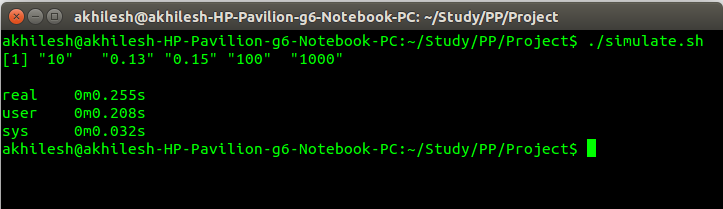
\includegraphics[scale=0.5]{1000}
\caption{Execution time for 1000 simulations}
\end{figure}
\begin{figure}[h]
\centering
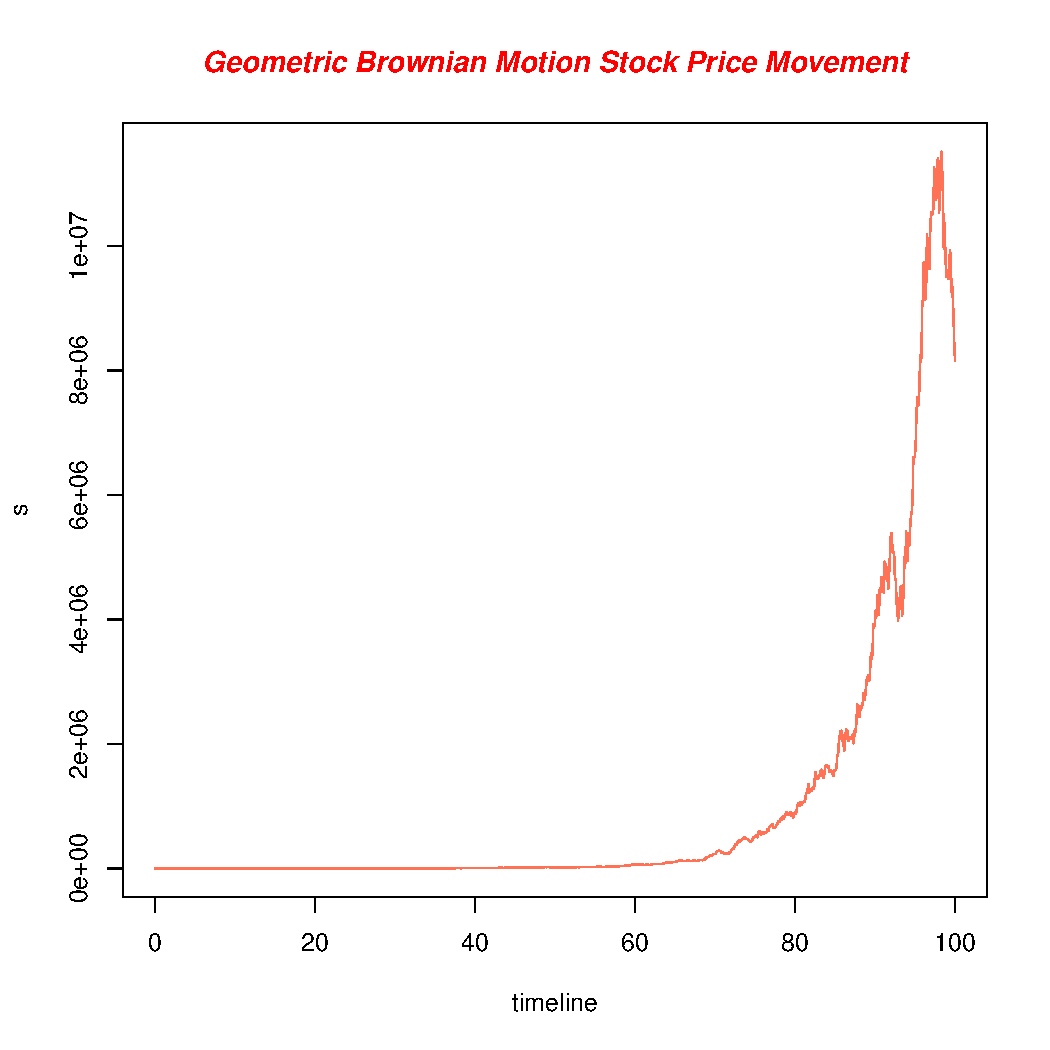
\includegraphics[scale=0.5]{1000_graph.pdf}
\caption{Brownian motion graph for 1000 simulations}
\end{figure}

\newpage
\item For 10000 simulations,\\
\begin{figure}[h]
\centering
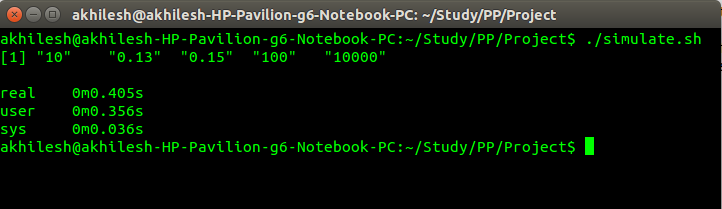
\includegraphics[scale=0.5]{10000}
\caption{Execution time for 10000 simulations}
\end{figure}
\begin{figure}[h]
\centering
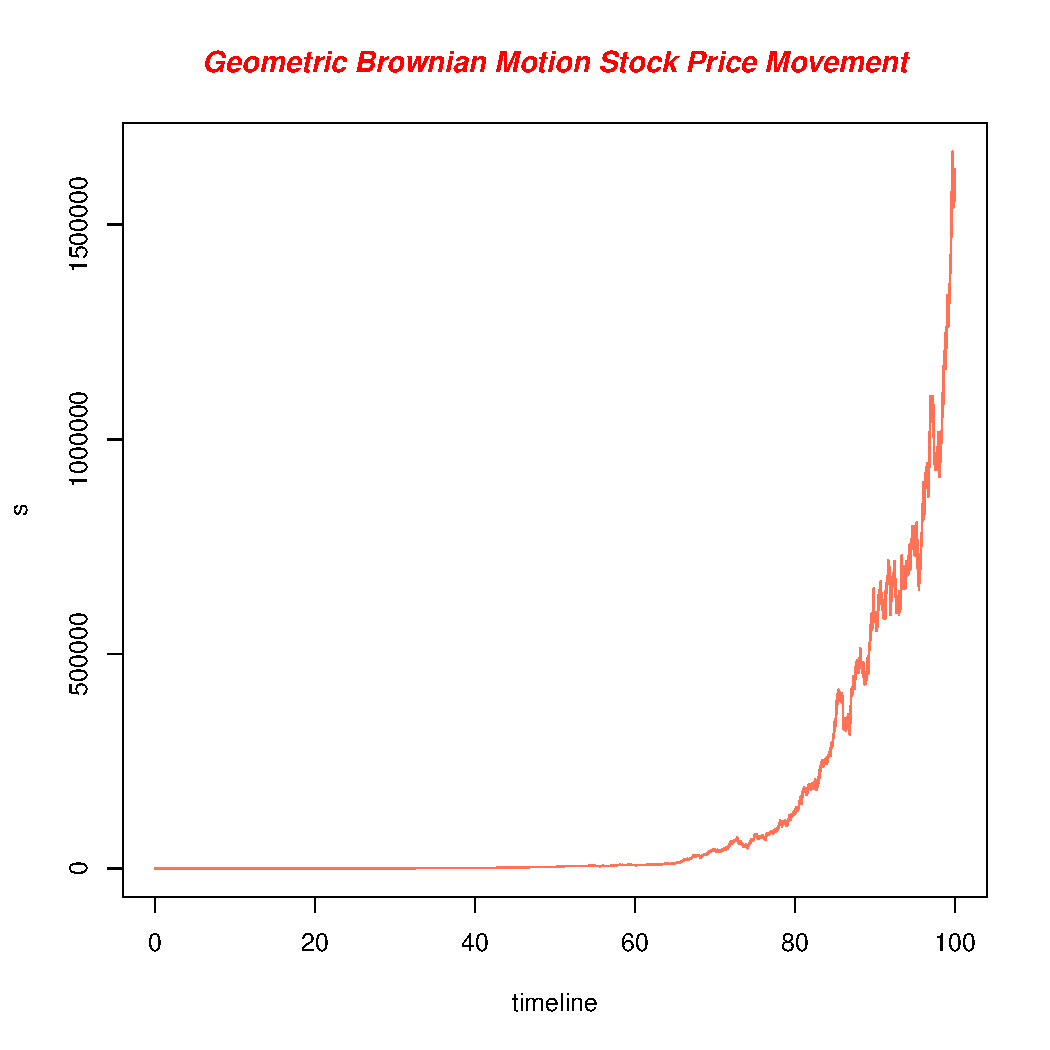
\includegraphics[scale=0.5]{10000_graph.pdf}
\caption{Brownian motion graph for 10000 simulations}
\end{figure}

\newpage
\item For 100000 simulations,\\
\begin{figure}[h]
\centering
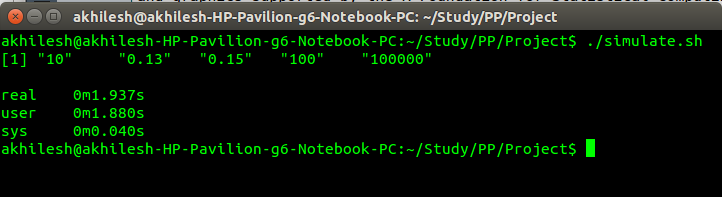
\includegraphics[scale=0.5]{100000}
\caption{Execution time for 100000 simulations}
\end{figure}
\begin{figure}[h]
\centering
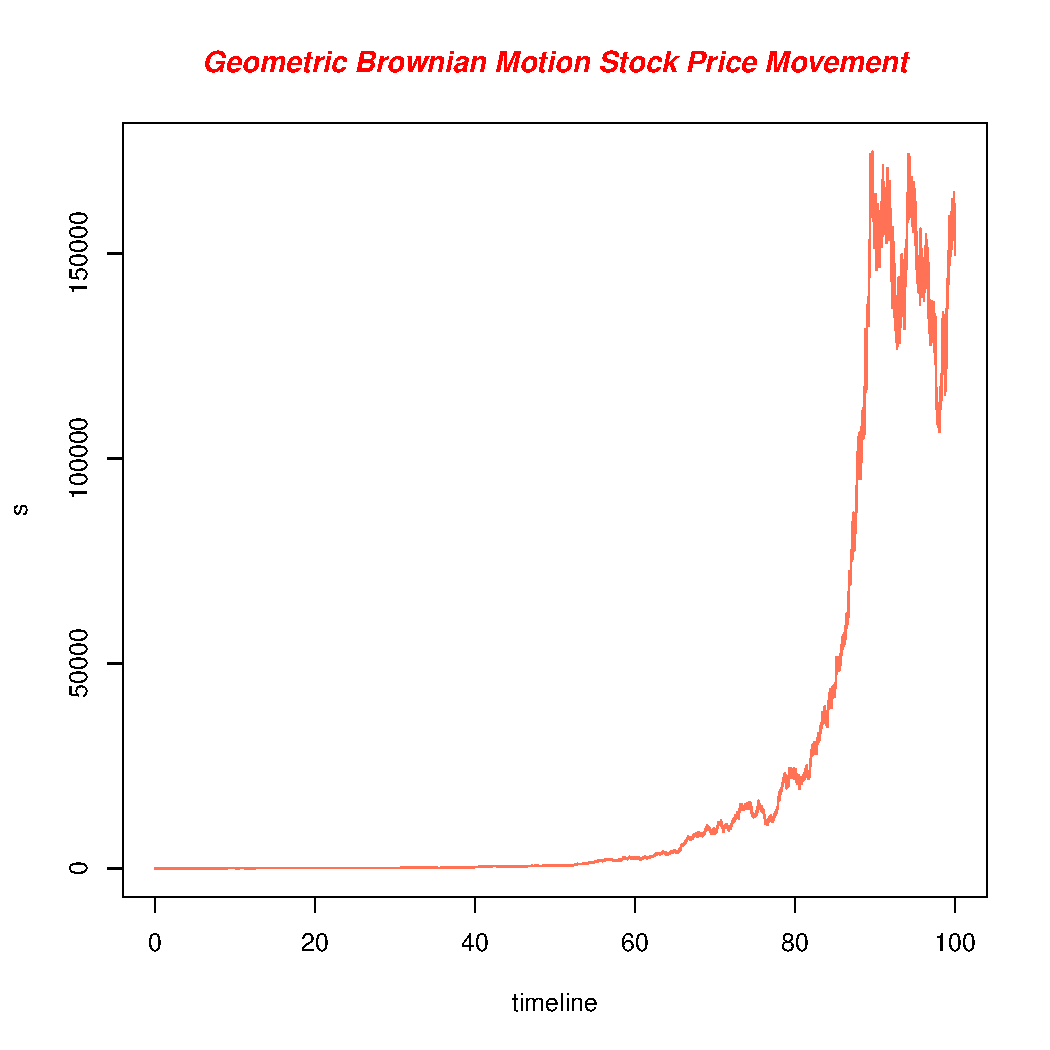
\includegraphics[scale=0.5]{100000_graph.pdf}
\caption{Brownian motion graph for 100000 simulations}
\end{figure}

\newpage
\item For 1000000 simulations,\\
\begin{figure}[h]
\centering
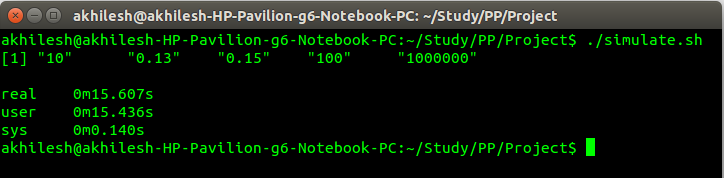
\includegraphics[scale=0.5]{1000000}
\caption{Execution time for 1000000 simulations}
\end{figure}
\begin{figure}[h]
\centering
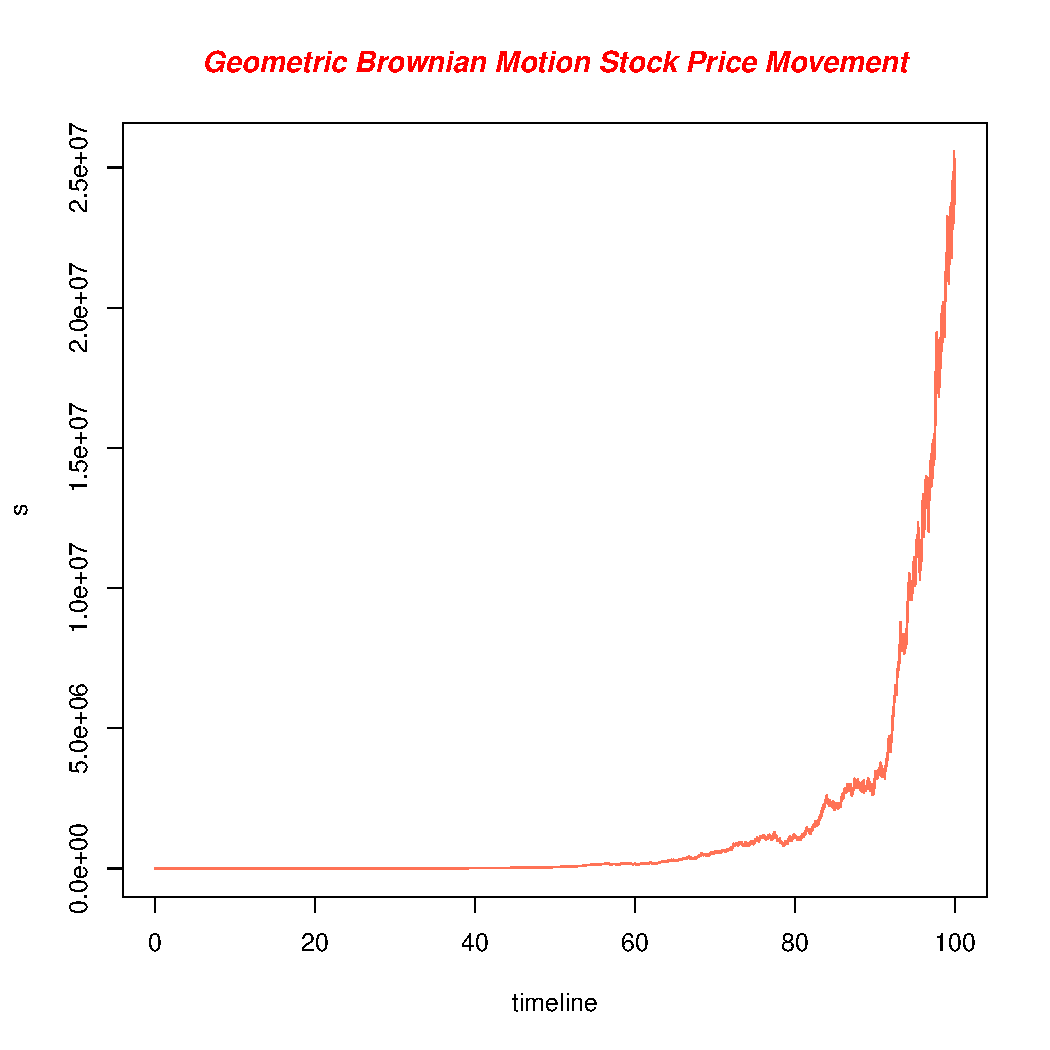
\includegraphics[scale=0.5]{1000000_graph.pdf}
\caption{Brownian motion graph for 1000000 simulations}
\end{figure}
\begin{figure}[H]
\centering
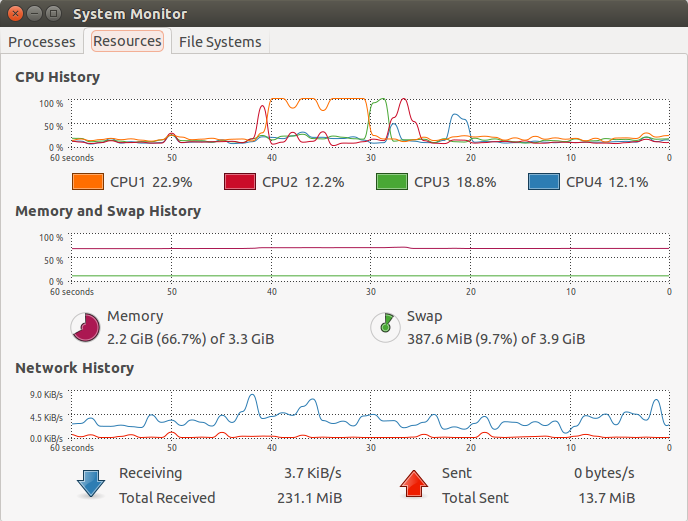
\includegraphics[scale=0.4]{1000000_sys_mon}
\caption{System Monitor for 1000000 simulations}
\end{figure}

\end{enumerate}
\newpage
\subsection{Outputs(Graphs and execution time for 'C')}
Given the parameters,\\
$S_{0}$, initial price of stock= 10,\\
$\mu$, expected return=13\%,\\
$\sigma$, standard  deviation of returns=15\%,\\
time, t=100
\begin{enumerate}
\item For 100 simulations,\\
\begin{figure}[h]
\centering
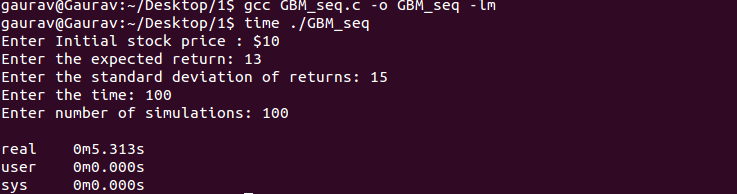
\includegraphics[scale=0.5]{100_SIM_GBM_SERIAL_C}
\caption{Execution time for 100 simulations}
\end{figure}

\item For 1000 simulations,\\
\begin{figure}[h]
\centering
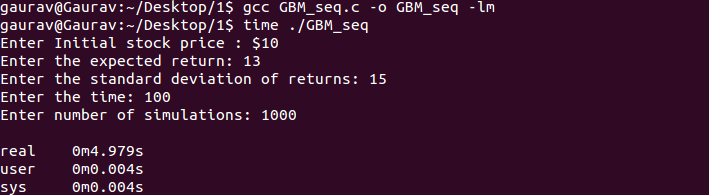
\includegraphics[scale=0.5]{1000_SIM_GBM_SERIAL_C}
\caption{Execution time for 1000 simulations}
\end{figure}

\newpage

\item For 10000 simulations,\\
\begin{figure}[h]
\centering
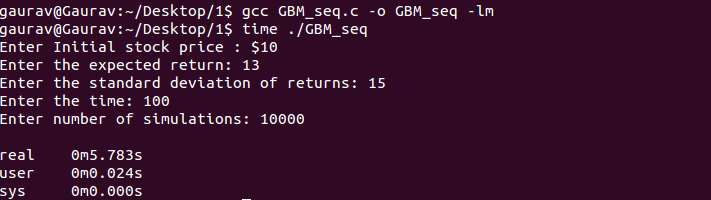
\includegraphics[scale=0.5]{10000_SIM_GBM_SERIAL_C}
\caption{Execution time for 10000 simulations}
\end{figure}

\item For 100000 simulations,\\
\begin{figure}[h]
\centering
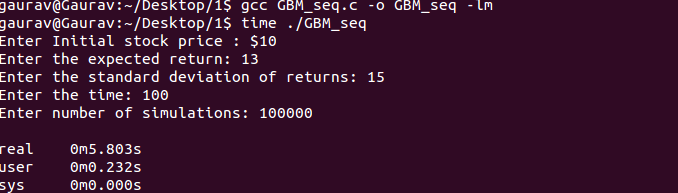
\includegraphics[scale=0.5]{100000_SIM_GBM_SERIAL_C}
\caption{Execution time for 100000 simulations}
\end{figure}

\item For 1000000 simulations,\\
\begin{figure}[h]
\centering
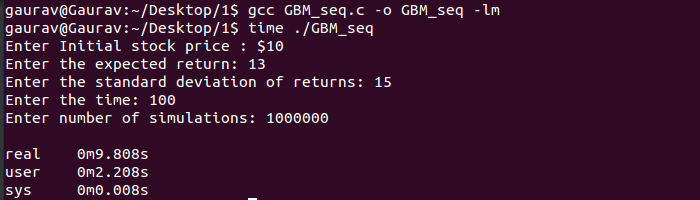
\includegraphics[scale=0.5]{1000000_SIM_GBM_SERIAL_C}
\caption{Execution time for 1000000 simulations}
\end{figure}

\begin{figure}[H]
\centering
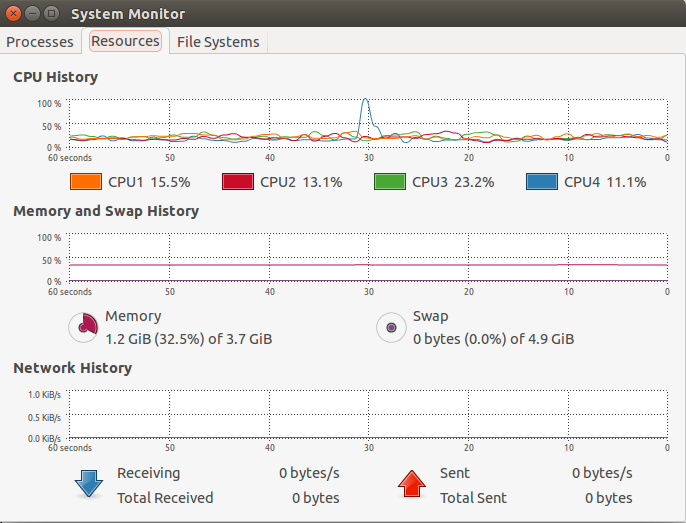
\includegraphics[scale=0.5]{CPU_usage_GBM_seq}
\caption{System Monitor for 1000000 simulations}
\end{figure}
\end{enumerate}

\subsubsection{Time Matrix for different number of simulations}
\begin{tabu} to 1.0\textwidth { | X[l] | X[c] | X[r] | X[l] | X[c] | X[r] |  }
 \hline
 Number of Iterations & 100 & 1000 & 10000 & 100000 & 1000000 \\
 \hline
 Time(In Seconds)  & 5.313  & 4.979 & 5.783 & 5.803 & 9.808  \\
\hline
\end{tabu}

\newpage
\subsubsection{Graph Between number of iterations and corresponding time taken}
\begin{figure}[h]
\centering
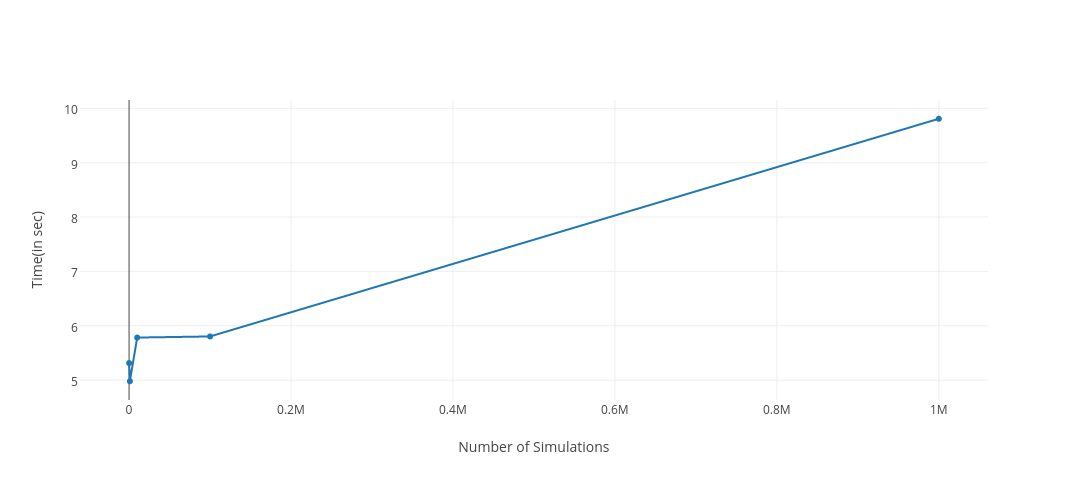
\includegraphics[scale=0.3]{Serial_graph}
\caption{Graph between Number of Simulations and Time(In seconds)}
\end{figure}

\subsubsection{Memory Allocation and Error Analysis}
\paragraph{Valgrind :}
It is a memory tool that will alert you about memory bugs and point you to where the problem might be. \\
\paragraph{Leaks vs Errors :}
Leaks occur when you allocate(malloc) memory that you fail to free and Errors occur when you attempt to read or write memory that you do not have access to (e.g. writing off the end of an array)\\ 
\begin{figure}[h]
\centering
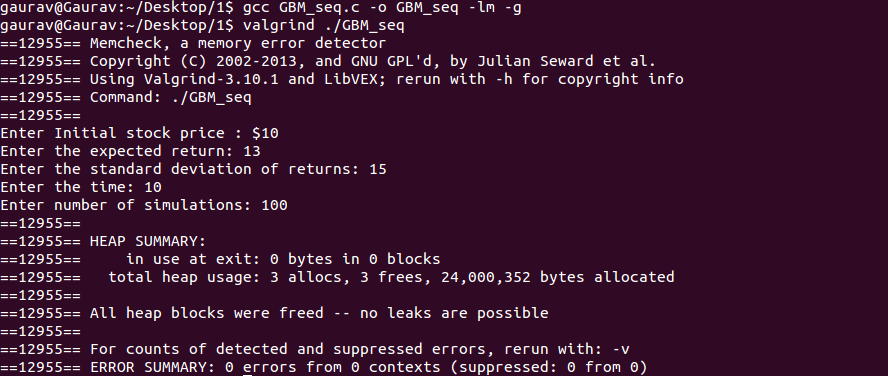
\includegraphics[scale=0.4]{Valgrind_GBM_seq_C}
\caption{Valgrind Memory Check Analysis of Serial Code}
\end{figure}
\newpage
\paragraph{Explanation:} 
There are Generally Two types of errors in memory check method\\ 
  (i)Invalid Read of size X(When we try to access a memory that we don't   
     have access to).\\
  (ii)Invalid write of size X(When we try to write into a memory that we 
      don't have access to)\\
In the serial code of GBM, we neither have any Invalid reads not Invalid     
writes(refer Figure 19).\\
\begin{figure}[h]
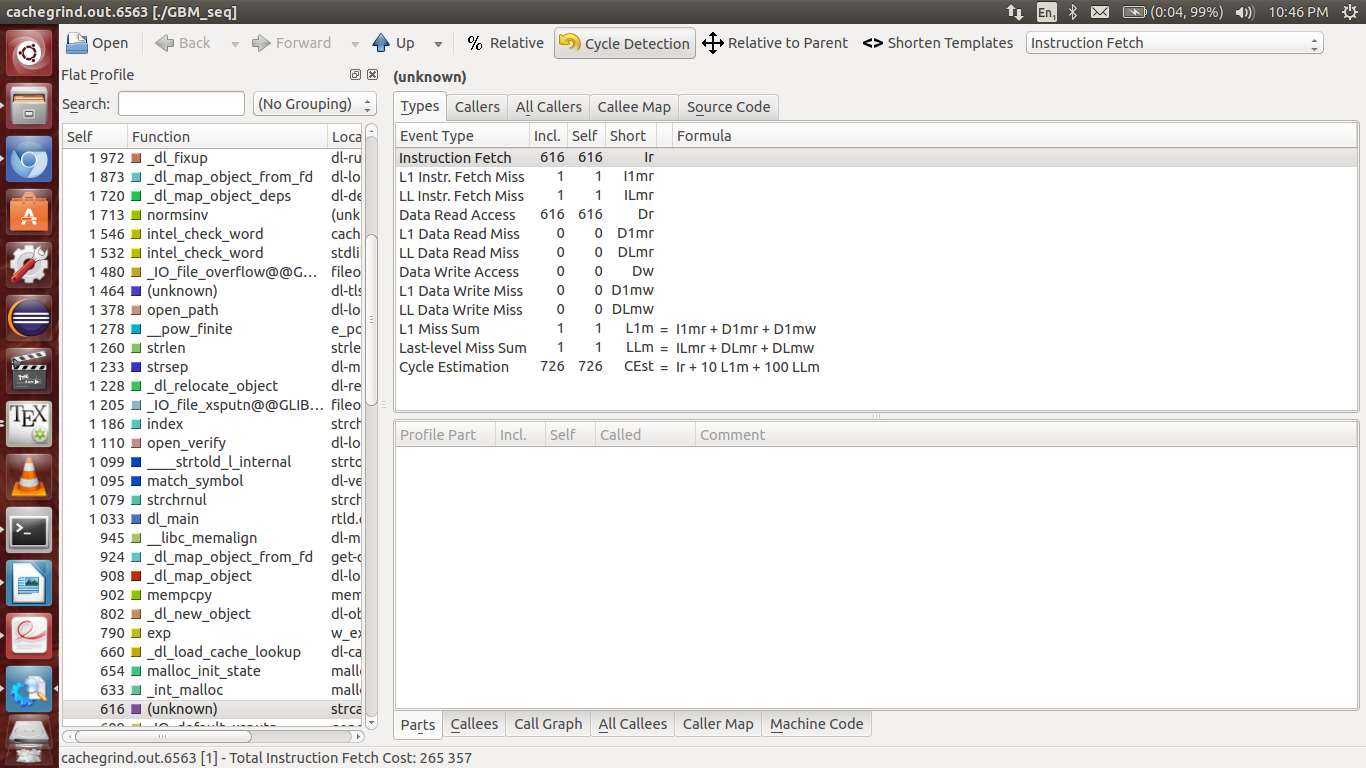
\includegraphics[scale=0.26]{k_cache_grind_serial}
\caption{KCache Grind Analysis of Serial code}
\end{figure}

\newpage
\section{Task Dependency Graph}
As There is only quantity that is being calculated for each simulation i.e. W(t).
\begin{figure}[h]
\centering
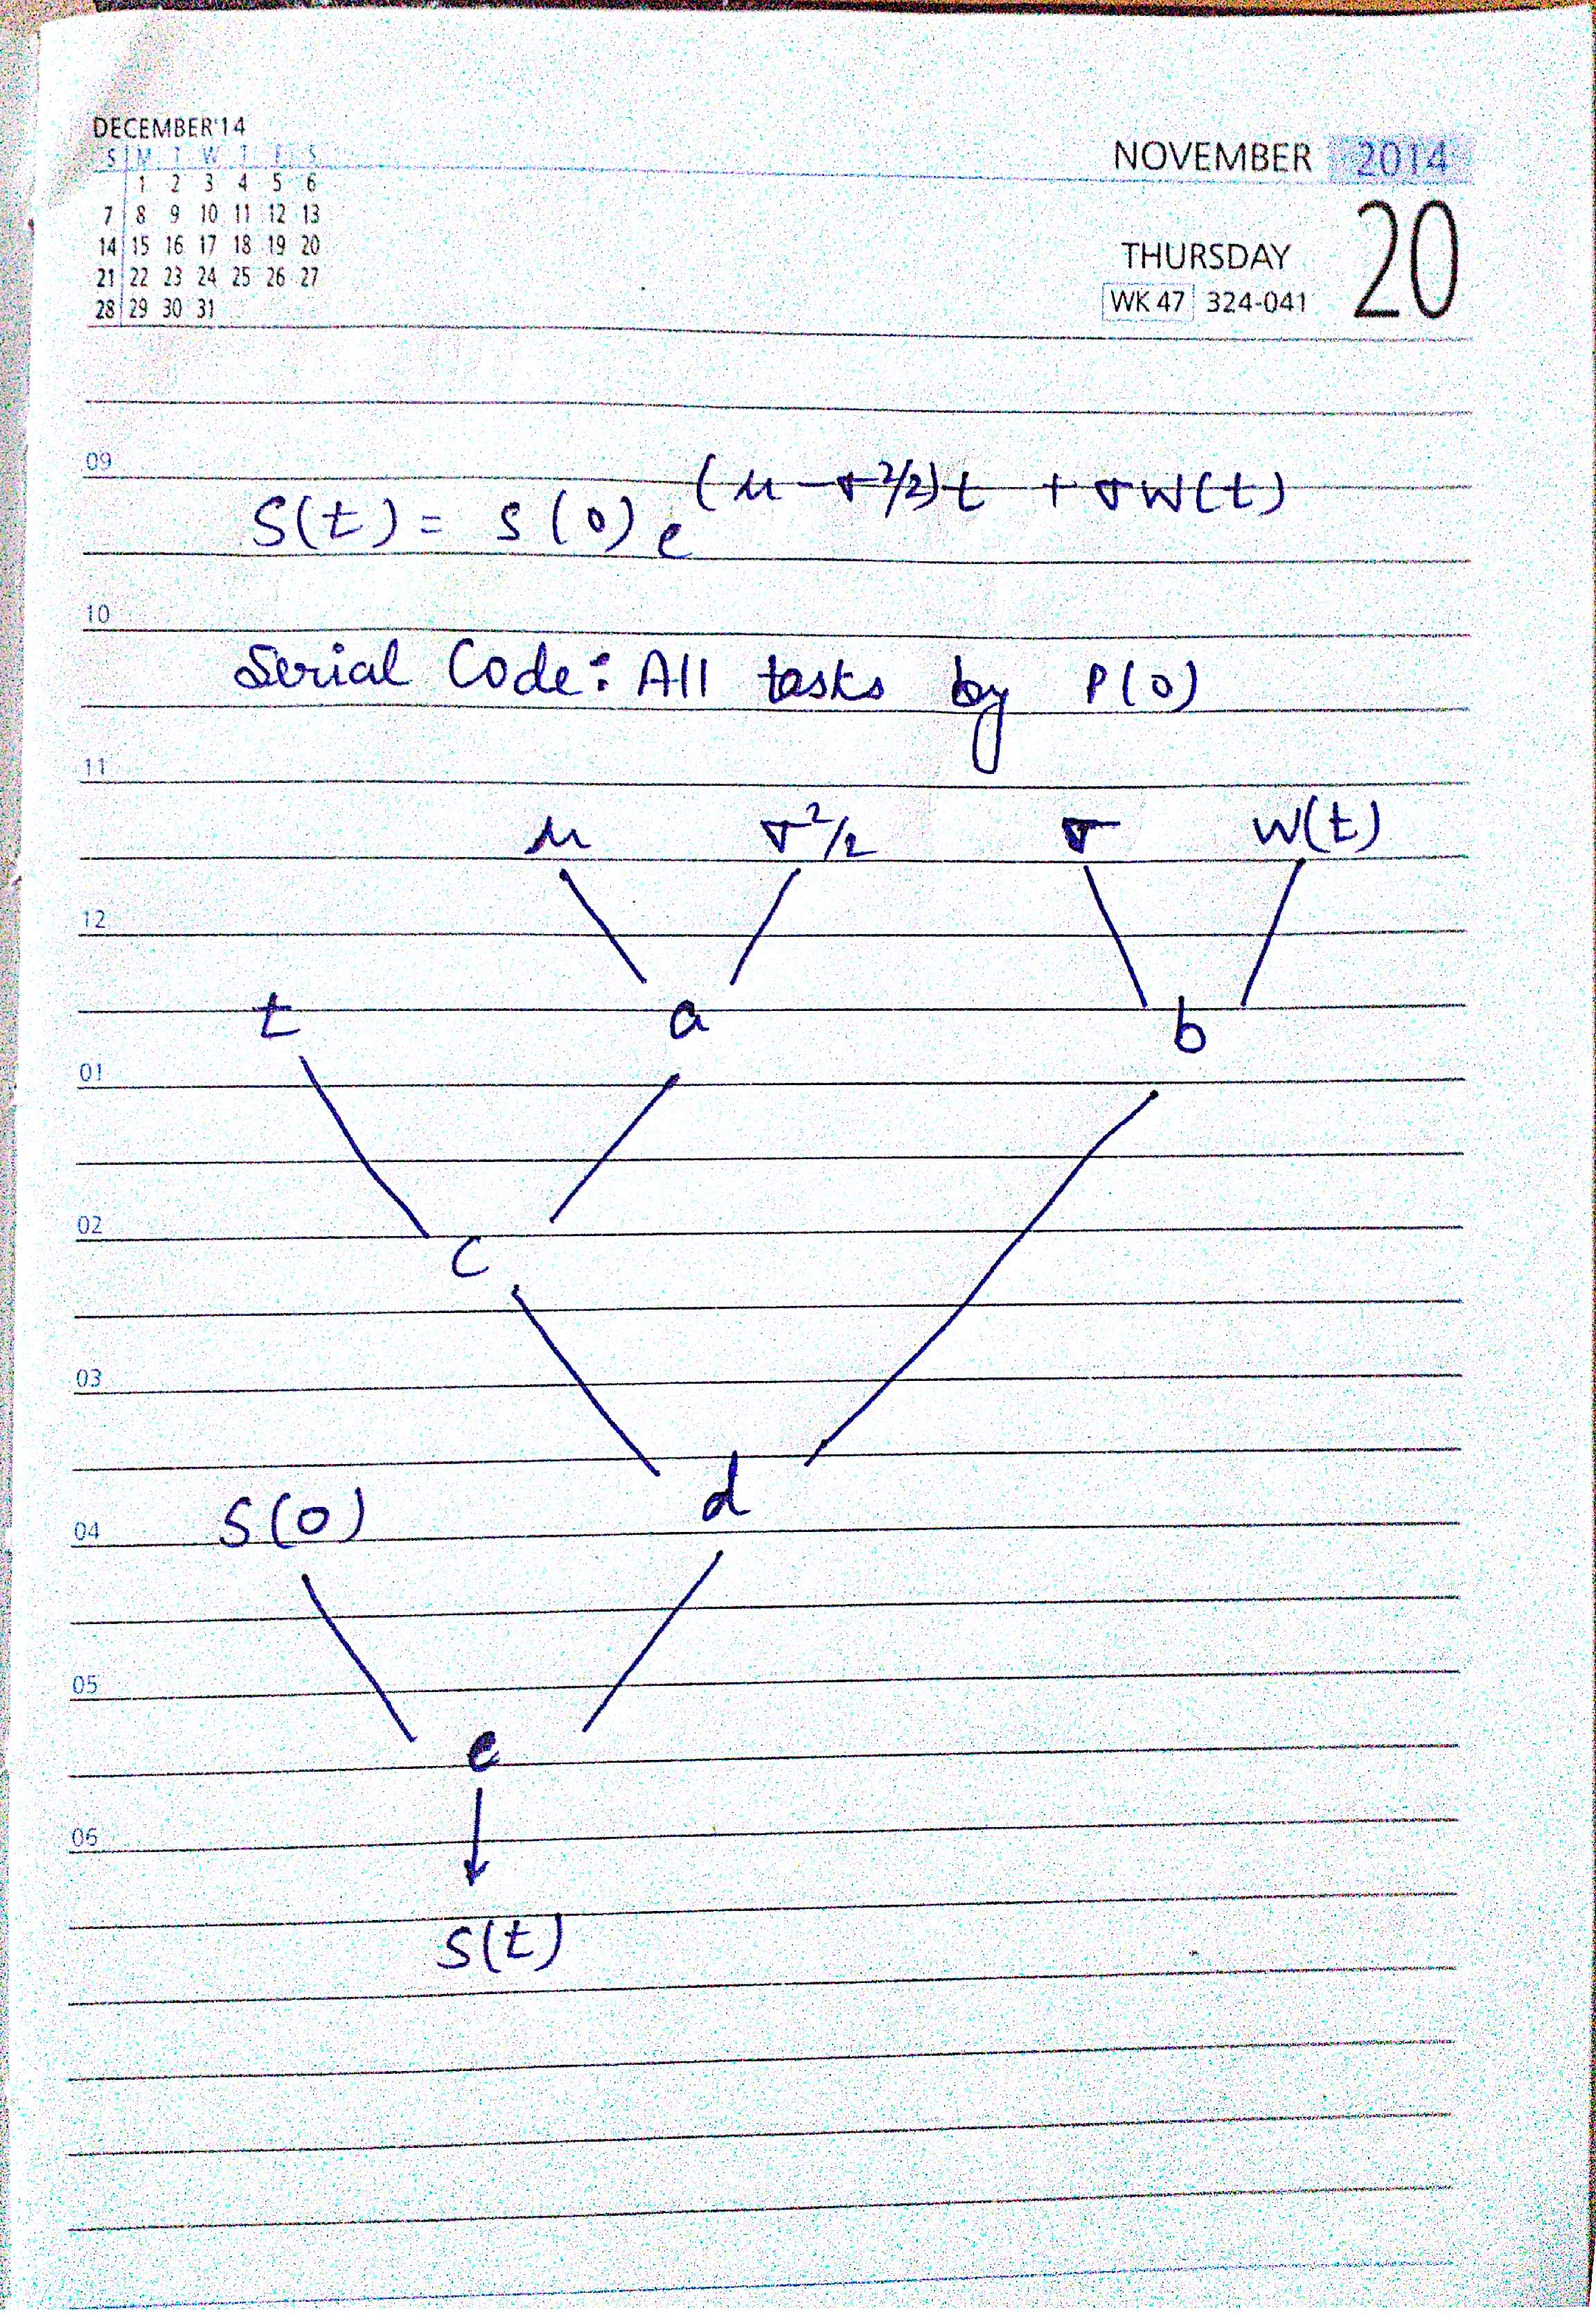
\includegraphics[scale=0.06]{Task_Dependency_Serial}
\caption{Task Dependency Graph for Serial Code}
\end{figure}


\newpage
\section{Conclusion}
We observe that with increasing number of simulations, execution time also increase. Also, we also observe that while executing the code for 10,00,000 simulations, one or two cores reach their 100\% processing power. This shows that other cores are idle and their execution capabilities are not utilized by the code. So, the code written is not optimised to utilize the full potential of the machine.

\section{Future/Concluding Work}
As of now, the code written is in R programming language. A serial code for this algorithm will be written in C and then will be evaluated for performance. After that, using parallel programming APIs like openMP, we will try to parallelize the code and com[ute the speedup. We can also compare whether for this kind of computational heavy algortihm, parallel code in C is better or serial code in R is better, performance wise. 

\section{Appendix}
\subsection{How to install R}
Run the following commands in your machine(OS: Ubuntu 14.04):
\begin{enumerate}
\item sudo sh -c 'echo "deb http://cran.rstudio.com/bin/linux/ubuntu trusty/" $\gg$ /etc/apt/sources.list'
\item gpg --keyserver keyserver.ubuntu.com --recv-key E084DAB9
\item gpg -a --export E084DAB9 | sudo apt-key add -
\item sudo apt-get update
\item sudo apt-get -y install r-base
\end{enumerate}
\subsection{How to run the code}
Attached are two files:
\begin{itemize}
\item GBMStock.R
\item simulate.sh
\end{itemize}
In the simulate.sh file, there are 5 args which are required by the R Script to run. The args stands for:\\
\begin{center}
GBMStock.R ``Initial Price of Stock" ``mu"" ``sigma"" ``Time"" ``Iterations""
\end{center}
In the terminal, run the \textbf{simulate.sh} file by manipulating the arguments and the output will be shown there. In the directory where the R Script is present, a new file ``Rplots.pdf" will be created with the corresponding graph in it.
\end{document}